
\section{Introduction}

Au cours des années, l’être humain a développé des moyens technologiques pour faciliter l'interaction avec les machines. À titre d’exemple l’humain a pratiquement remplacé l’utilisation du clavier par la voix. Des assistants intelligents effectuent la plupart des tâches sur nos ordinateurs et nos Smart phones.
\\Lorsque nous parlons d'assistants intelligents, ceux-ci doivent être capables de comprendre l'énoncé de l'utilisateur, le transformer en requête et y produire une réponse ou action. \\ \\Au cours de ce chapitre, nous aborderons en détail les principes de base de la reconnaissance automatique de la parole et des systèmes de questions réponses.

\section{Reconnaissance de la parole (Speech to text)}
\subsection{Définition}
Le Speech Recognition (ou reconnaissance de la parole en français) est la capacité d'une machine à comprendre des mots parlés. Un microphone enregistre la voix d'une personne et le matériel convertit le signal d'ondes sonores analogiques en audio numérique. Les données audio sont ensuite traitées par un logiciel, qui interprète les mots. \cite{speechrecdef}
\newpage
\subsection{Historique}
La parole est le principal moyen de communication entre les personnes et pour cette raison le domaine de la reconnaissance de la parole a attiré beaucoup d’attention au cours des six dernières décennies. Les premières expérimentations virent le jour au cours des années 50 avec le système “Audrey” en 1952 qui reconnaissait des chiffres émis par une unique voix. En 1962 IBM présente “Shoebox”, un système permettant de reconnaître 16 mots de la langue anglaise.\\
Malgré ces premières avancées, c’est dans les années 70 que ce domaine décolle réellement avec le système militaire “Harpy” qui pouvait comprendre  1011 mots, ce qui représentait le vocabulaire d’un enfant de 3 ans.\\
Les années 80 furent marquées par l’utilisation d’une nouvelle méthode “Modèle de Markov Caché” (sera abordé en détail dans la suite de ce chapitre) afin de prédire et comprendre les mots, ce qui en théorie permettait de prédire un nombre illimité de mots et si ce n'était pas le cas en pratique à cette époque là, ça le fut les deux décennies suivantes.\cite{speechrechist}
\\
Les systèmes de reconnaissance de la parole n’ont cessé de se perfectionner au cours des années 90 et 2000. Avec l'avènement de Google en 2001, ces systèmes se vantaient d’une précision de 80\% et n’a cessé d'accroître.\cite{audreysiri}
\\ \\Il est important d'ajouter que ce ne sont pas que les performances de ces systèmes qui ont évolué au fil des décennies mais également les paramètres que nous prenons en compte lors de la reconnaissance de la parole.\\
Alors qu'à ses débuts, la reconnaissance de la parole ne pouvait donner de résultat que si nous avions : un petit, vocabulaire, une requête élémentaire bien définie, un environnement propre sans bruit, une prononciation académique et une seule langue, nos systèmes sont aujourd'hui capables de faire de la reconnaissance sous tout type de condition comme le montre la figure suivante : 

\begin{figure}[H]
    \centering
    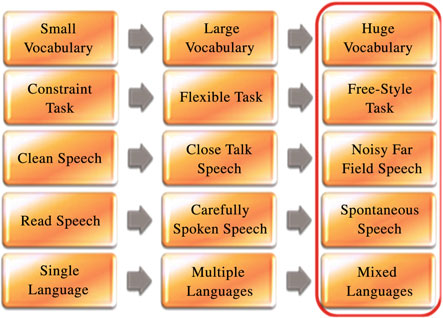
\includegraphics[height=200pt,width=300pt]{images/chap1/evolution.png}
    \caption{Évolution des contraintes lors de la reconnaissance de la parole\cite{deeplearningapproach}}
\end{figure}

\subsection{Utilisation de ces systèmes}
Le fait que la reconnaissance de la parole ait suscité autant d'intérêt ces dernières décennies n’est pas dû au hasard. En effet ces systèmes sont d’une très grande utilité tant pour améliorer la communication entre les humains mais aussi et surtout la communication entre l’humain et la machine.\cite{deeplearningapproach}
\\Les systèmes de reconnaissance de la parole peuvent avoir les applications suivantes : 
\begin{itemize}
    \item Permettre de faciliter la traduction lors de la communication avec des gens qui parlent une langue différente.
    \item Les assistants intelligents basés sur la reconnaissance de la parole sont de nos jours présents dans beaucoup d’appareils électroniques permettant ainsi de rendre nos tâches du quotidien plus simples à réaliser.
    \item Permettre à l'utilisateur d'exprimer des requêtes en langage naturel sans avoir à passer par un clavier réduisant ainsi considérablement le temps et les efforts de l'utilisateur.
\end{itemize}

\subsection{Architecture}
Les systèmes de reconnaissance de la paroles partagent une architecture commune et ce indépendamment de la langue traitée.
\\Cette architecture comporte quatre modules principaux qui sont représentés dans le diagramme suivant :
\begin{figure}[H]
    \centering
    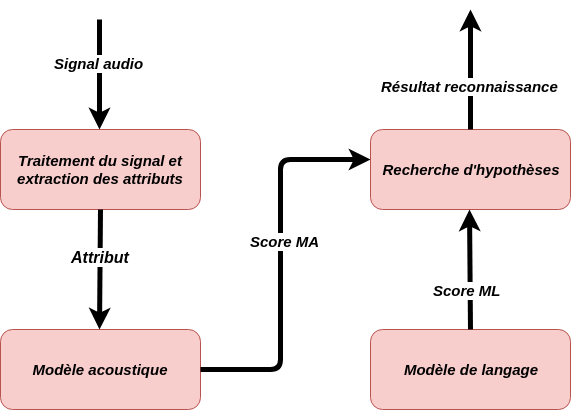
\includegraphics[height=200pt,width=300pt]{images/chap1/architecture_asr.png}
    \caption{Architecture système de reconnaissance de la parole\cite{deeplearningapproach}}
\end{figure}

Nous décrivons dans ce qui suit chaque module de l'architecture :
\newpage
\subsubsection{Traitement du signal et extraction des attributs}
Traduit de "signal processing and feature extraction", ce module de l’architecture va prendre notre audio qui en entrée, passer par une étape de réduction du bruit, transformation du signal en fréquences et envoie de vecteurs de caractéristiques au prochain module du système.

\subsubsection{Modèle acoustique}
Qui représente la base de l'architecture et a pour objectif de transformer les informations contenues dans le vecteurs de caractéristiques en unités linguistiques qui seront par la suite traitées au niveau du module suivant. Plusieurs approches ont été utilisées pour répondre à ce besoin :\cite{featureextract}
\begin{itemize}
    \item approches terministiques également appelées algorithmes dynamiques de déformation temporelle. C’est une Ancienne approche, très rarement utilisé de nos jours. \cite{terministicapproach}
    \item Approche statistique, nous parlons ici de HMM\footnote{Hidden Markov Models, notion qui sera traitée en détail par la suite.} et de GMM\footnote{Gaussian Mixture Model, notion qui sera traitée en détail par la suite.} mais aussi de modèles d’apprentissage profond ou encore des modèles hybrides HMM-DNN\footnote{Deep Neural Networks : réseaux de neurons profonds, notion qui sera traitée en détail par la suite.}.	 
\end{itemize}

\subsubsection{Modèle de langage}
Utilisé dans les systèmes de reconnaissance de la parole et systèmes de traduction automatique pour améliorer leur performance. En pratique, ce modèle est utilisé pour rechercher une interprétation de l'entrée du modèle acoustique et prédire une suite de mots correspondants à cette entrée. Ce modèle peut être basé sur :\cite{languagemodel}
\\
\begin{itemize}
    \item Une grammaire : Utilisé généralement lorsque la gamme de phrases à reconnaître est très petite et peut être capturée par une grammaire déterministe, autrement dit, très peu utilisé de nos jours. 
    \item Un modèle probabiliste, nous parlons ici de la notion de N-Grammes qui sera détaillée par la suite. 
\end{itemize}

\subsubsection{Recherche d'hypothèses}
Pour le modèle acoustique et modèle de langue, un score est généré pour évaluer le résultat et c’est ce score qui est utilisé lors de la recherche d’hypothèses.\\
Ce module  Combine les différents scores obtenus à travers les deux modules précédents étant donné la séquence de vecteur de caractéristiques et affiche la séquence de mots avec le score le plus élevé comme résultat de la reconnaissance.\cite{deeplearningapproach}

\section{Les système les plus performants}
Toutes les grandes compagnies de l’industrie des nouvelles technologies se sont tournés vers les systèmes de reconnaissance de la parole et ont produits différents outils à cet effet.\\
Il existe plusieurs API\footnote{Application Programming Interface : ensemble normalisé de classes, de méthodes ou de fonctions qui sert de façade par laquelle un logiciel offre des services à d'autres logiciels} permettant de faire de la reconnaissance de la parole, nous présentons une étude dans ce qui suit trois des systèmes les plus performants :\cite{compareapi} \\
\begin{itemize}
    \item \textbf{CMU SPHINX} : Le système Sphinx a été développé à l’université Carnegie Mellon (CMU). Au cours du développement plusieurs versions ont vu le jour tel que Sphinx-2 Sphinx-3, Sphinx-4, Pocketsphinx, Sphinxbase et Sphinxtrain. Pour cette comparaison nous choisissons Sphinx-4 pour son vocabulaire important et la flexibilité qu’il apporte.
    \item \textbf{Google API} : En utilisant de l’apprentissage profond (Deep Learning), Google a pu avoir un taux d'erreur de 8\% en 2015 comparé à 23\% de 2013 ce qui fait de l’API de Google un candidat idéal pour notre comparaison.
    \item \textbf{Microsoft API} : Depuis 1993 Microsoft n’a cessé de développer son API de reconnaissance de la parole et a produit des applications performantes.
\end{itemize}

Cette étude fut menée sur ces trois systèmes en se basant sur le Timit corpus\cite{timit}.
\\ \\ Afin d'évaluer un système de reconnaissance de la parole, nous utilisons la métrique WER\footnote{Word Error Rate ou taux d'erreur des mots} qui est représenté par la formule suivante\cite{werformula} : \\
\begin{equation}
    WER = \frac{S + D + I}{N}
\end{equation}
\\    
Les résultats de l'étude furent les suivants : 
\begin{itemize}
    \item 8\% pour l'API Google.
    \item 18\% pour l'API Microsoft.
    \item 37\% pour le CMU SPHINX.
\end{itemize}
De nos jours, l'API Google est celle qui présente les meilleures performances, cependant elle ne présente pas des résultats satisfaisants pour la langue arabe.

\newpage
\section{Systèmes de synthèse vocale}
\subsection{Présentation}
Les systèmes de synthèse vocale\footnote{Text to speech en anglais} sont utilisés pour convertir des mots écrits (dans un document par exemple) en discours audible, ces systèmes doivent êtres capables de lire n'importe quel texte qui puisse être prononcé.\\
Les systèmes de synthèse vocale se basent sur deux parties principales, conversion du texte en phonèmes pour ensuite convertir les caractéristiques linguistiques des phonèmes en parole\cite{textspeechpres}
\\ \\
Ces systèmes sont largement utilisés de nos jours et il y a de plus en plus d'applications fournissant des services de synthèse vocale pour les possibilités que ceux-ci offrent, nous pouvons citer : 
\begin{itemize}
    \item L’aide aux mal-voyants.
    \item Aide à la traduction et à la prononciation.
    \item Nouvelle dimension pour les assistants intelligents.
\end{itemize}

\subsection{Architecture}
Un système de synthèse vocale doit être composé des modules suivants : \cite{textspeechmodules}

\begin{itemize}
    \item \textbf{Conversion de graphème vers phonèmes} : Permet de convertir un texte écrit en phonèmes en utilisant un alphabet phonétique (comme le Arpabet\cite{arpabet} par exemple).
    \item \textbf{Modèle de segmentation} : localise les limites des phonèmes dans le jeu de données de voix. Ce modèle nous permet donc de connaître dans une séquence audio le début et la fin d’un phonème.
    \item \textbf{Modèle de durée de phonème} : prédit la durée de chaque phonème dans une séquence de phonèmes.
    \item \textbf{Modèle de fréquence fondamentale} :  Prédit si un phonème est exprimé et si tel est le cas il retourne la fréquence de base de ce phonème selon la durée de ce dernier.
    \item \textbf{Modèle de synthèse audio} : Combine les sorties des modèles précédents et nous donne en sortie une synthèse vocale du texte désiré.
\end{itemize}

\newpage
La figure résume l'architecture des systèmes de synthèse vocale.

\begin{figure}[H]
    \centering
    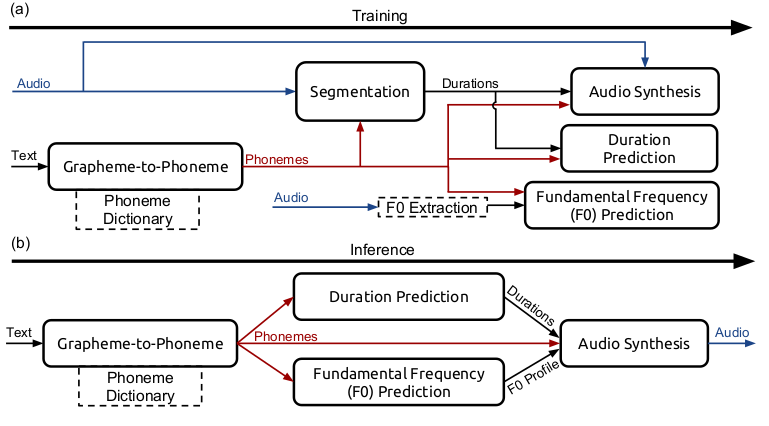
\includegraphics[height=200pt,width=300pt]{images/chap1/architecture_tts.png}
    \caption{Architecture système de synthèse vocale\cite{textspeechmodules}}
\end{figure}